% Created by tikzDevice version 0.12.6 on 2025-05-06 20:55:50
% !TEX encoding = UTF-8 Unicode
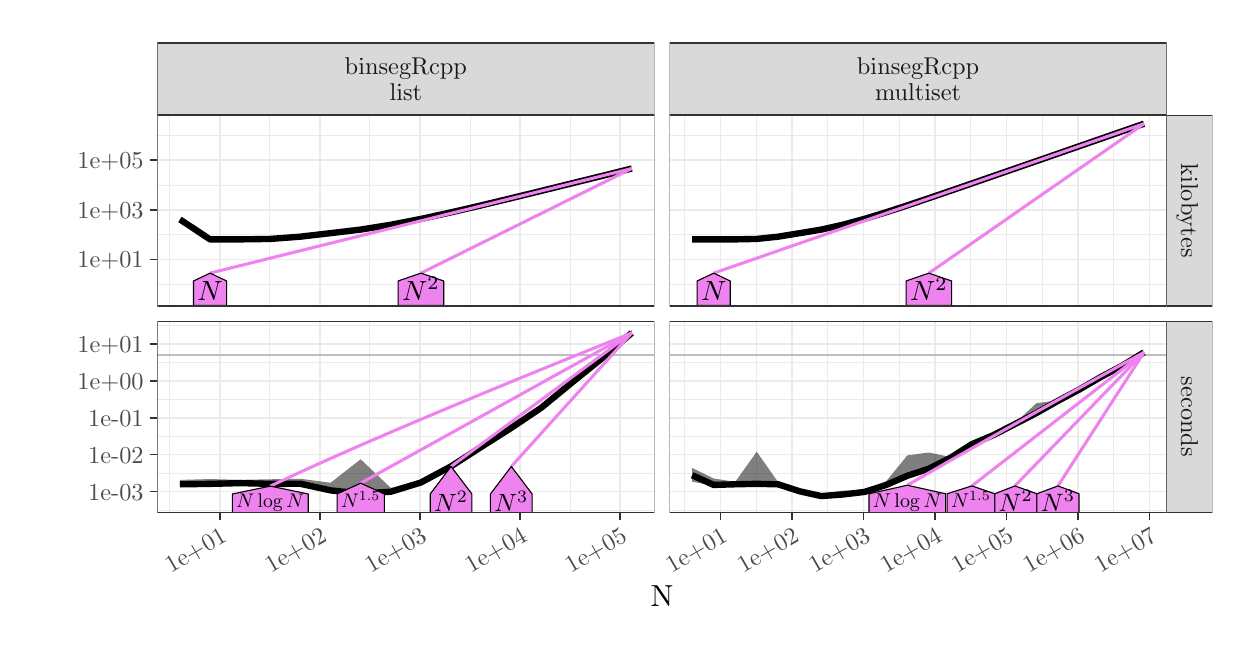
\begin{tikzpicture}[x=1pt,y=1pt]
\definecolor{fillColor}{RGB}{255,255,255}
\path[use as bounding box,fill=fillColor,fill opacity=0.00] (0,0) rectangle (433.62,216.81);
\begin{scope}
\path[clip] (  0.00,  0.00) rectangle (433.62,216.81);
\definecolor{drawColor}{RGB}{255,255,255}
\definecolor{fillColor}{RGB}{255,255,255}

\path[draw=drawColor,line width= 0.6pt,line join=round,line cap=round,fill=fillColor] ( -0.00,  0.00) rectangle (433.62,216.81);
\end{scope}
\begin{scope}
\path[clip] ( 46.86,116.18) rectangle (226.46,185.23);
\definecolor{fillColor}{RGB}{255,255,255}

\path[fill=fillColor] ( 46.86,116.18) rectangle (226.46,185.23);
\definecolor{drawColor}{gray}{0.92}

\path[draw=drawColor,line width= 0.3pt,line join=round] ( 46.86,124.04) --
	(226.46,124.04);

\path[draw=drawColor,line width= 0.3pt,line join=round] ( 46.86,141.98) --
	(226.46,141.98);

\path[draw=drawColor,line width= 0.3pt,line join=round] ( 46.86,159.91) --
	(226.46,159.91);

\path[draw=drawColor,line width= 0.3pt,line join=round] ( 46.86,177.84) --
	(226.46,177.84);

\path[draw=drawColor,line width= 0.3pt,line join=round] ( 51.34,116.18) --
	( 51.34,185.23);

\path[draw=drawColor,line width= 0.3pt,line join=round] ( 87.49,116.18) --
	( 87.49,185.23);

\path[draw=drawColor,line width= 0.3pt,line join=round] (123.65,116.18) --
	(123.65,185.23);

\path[draw=drawColor,line width= 0.3pt,line join=round] (159.81,116.18) --
	(159.81,185.23);

\path[draw=drawColor,line width= 0.3pt,line join=round] (195.97,116.18) --
	(195.97,185.23);

\path[draw=drawColor,line width= 0.6pt,line join=round] ( 46.86,133.01) --
	(226.46,133.01);

\path[draw=drawColor,line width= 0.6pt,line join=round] ( 46.86,150.94) --
	(226.46,150.94);

\path[draw=drawColor,line width= 0.6pt,line join=round] ( 46.86,168.88) --
	(226.46,168.88);

\path[draw=drawColor,line width= 0.6pt,line join=round] ( 69.42,116.18) --
	( 69.42,185.23);

\path[draw=drawColor,line width= 0.6pt,line join=round] (105.57,116.18) --
	(105.57,185.23);

\path[draw=drawColor,line width= 0.6pt,line join=round] (141.73,116.18) --
	(141.73,185.23);

\path[draw=drawColor,line width= 0.6pt,line join=round] (177.89,116.18) --
	(177.89,185.23);

\path[draw=drawColor,line width= 0.6pt,line join=round] (214.04,116.18) --
	(214.04,185.23);
\definecolor{drawColor}{RGB}{0,0,0}

\path[draw=drawColor,line width= 2.3pt,line join=round] ( 55.03,147.52) --
	( 65.91,140.30) --
	( 76.80,140.31) --
	( 87.68,140.47) --
	( 98.56,141.29) --
	(109.45,142.56) --
	(120.33,143.85) --
	(131.22,145.59) --
	(142.10,147.70) --
	(152.99,150.07) --
	(163.87,152.59) --
	(174.76,155.20) --
	(185.64,157.85) --
	(196.52,160.53) --
	(207.41,163.21) --
	(218.29,165.91);
\definecolor{drawColor}{RGB}{238,130,238}

\path[draw=drawColor,line width= 1.1pt,line join=round] (142.10,128.12) --
	(152.99,133.52) --
	(163.87,138.92) --
	(174.76,144.31) --
	(185.64,149.71) --
	(196.52,155.11) --
	(207.41,160.51) --
	(218.29,165.91);

\path[draw=drawColor,line width= 1.1pt,line join=round] ( 65.91,128.12) --
	( 76.80,130.82) --
	( 87.68,133.52) --
	( 98.56,136.22) --
	(109.45,138.92) --
	(120.33,141.62) --
	(131.22,144.31) --
	(142.10,147.01) --
	(152.99,149.71) --
	(163.87,152.41) --
	(174.76,155.11) --
	(185.64,157.81) --
	(196.52,160.51) --
	(207.41,163.21) --
	(218.29,165.91);
\end{scope}
\begin{scope}
\path[clip] ( 46.86,116.18) rectangle (226.46,185.23);
\definecolor{drawColor}{RGB}{0,0,0}
\definecolor{fillColor}{RGB}{238,130,238}

\path[draw=drawColor,line width= 0.4pt,line join=round,line cap=round,fill=fillColor] (133.87,125.28) --
	(142.10,128.12) --
	(150.33,125.28) --
	(150.33,116.41) --
	(133.87,116.41) --
	cycle;

\path[draw=drawColor,line width= 0.4pt,line join=round,line cap=round,fill=fillColor] ( 59.93,125.28) --
	( 65.91,128.12) --
	( 71.90,125.28) --
	( 71.90,116.41) --
	( 59.93,116.41) --
	cycle;

\node[text=drawColor,anchor=base,inner sep=0pt, outer sep=0pt, scale=  1.00] at (142.10,118.39) {$N^2$};

\node[text=drawColor,anchor=base,inner sep=0pt, outer sep=0pt, scale=  1.00] at ( 65.91,118.39) {$N$};
\definecolor{drawColor}{gray}{0.20}

\path[draw=drawColor,line width= 0.6pt,line join=round,line cap=round] ( 46.86,116.18) rectangle (226.46,185.23);
\end{scope}
\begin{scope}
\path[clip] ( 46.86, 41.62) rectangle (226.46,110.68);
\definecolor{fillColor}{RGB}{255,255,255}

\path[fill=fillColor] ( 46.86, 41.62) rectangle (226.46,110.68);
\definecolor{drawColor}{gray}{0.92}

\path[draw=drawColor,line width= 0.3pt,line join=round] ( 46.86, 42.48) --
	(226.46, 42.48);

\path[draw=drawColor,line width= 0.3pt,line join=round] ( 46.86, 55.84) --
	(226.46, 55.84);

\path[draw=drawColor,line width= 0.3pt,line join=round] ( 46.86, 69.20) --
	(226.46, 69.20);

\path[draw=drawColor,line width= 0.3pt,line join=round] ( 46.86, 82.55) --
	(226.46, 82.55);

\path[draw=drawColor,line width= 0.3pt,line join=round] ( 46.86, 95.91) --
	(226.46, 95.91);

\path[draw=drawColor,line width= 0.3pt,line join=round] ( 46.86,109.27) --
	(226.46,109.27);

\path[draw=drawColor,line width= 0.3pt,line join=round] ( 51.34, 41.62) --
	( 51.34,110.68);

\path[draw=drawColor,line width= 0.3pt,line join=round] ( 87.49, 41.62) --
	( 87.49,110.68);

\path[draw=drawColor,line width= 0.3pt,line join=round] (123.65, 41.62) --
	(123.65,110.68);

\path[draw=drawColor,line width= 0.3pt,line join=round] (159.81, 41.62) --
	(159.81,110.68);

\path[draw=drawColor,line width= 0.3pt,line join=round] (195.97, 41.62) --
	(195.97,110.68);

\path[draw=drawColor,line width= 0.6pt,line join=round] ( 46.86, 49.16) --
	(226.46, 49.16);

\path[draw=drawColor,line width= 0.6pt,line join=round] ( 46.86, 62.52) --
	(226.46, 62.52);

\path[draw=drawColor,line width= 0.6pt,line join=round] ( 46.86, 75.88) --
	(226.46, 75.88);

\path[draw=drawColor,line width= 0.6pt,line join=round] ( 46.86, 89.23) --
	(226.46, 89.23);

\path[draw=drawColor,line width= 0.6pt,line join=round] ( 46.86,102.59) --
	(226.46,102.59);

\path[draw=drawColor,line width= 0.6pt,line join=round] ( 69.42, 41.62) --
	( 69.42,110.68);

\path[draw=drawColor,line width= 0.6pt,line join=round] (105.57, 41.62) --
	(105.57,110.68);

\path[draw=drawColor,line width= 0.6pt,line join=round] (141.73, 41.62) --
	(141.73,110.68);

\path[draw=drawColor,line width= 0.6pt,line join=round] (177.89, 41.62) --
	(177.89,110.68);

\path[draw=drawColor,line width= 0.6pt,line join=round] (214.04, 41.62) --
	(214.04,110.68);
\definecolor{drawColor}{RGB}{190,190,190}

\path[draw=drawColor,line width= 0.6pt,line join=round] ( 46.86, 98.57) -- (226.46, 98.57);
\definecolor{fillColor}{RGB}{0,0,0}

\path[fill=fillColor,fill opacity=0.50] ( 55.03, 53.39) --
	( 65.91, 53.70) --
	( 76.80, 53.42) --
	( 87.68, 53.62) --
	( 98.56, 53.81) --
	(109.45, 52.36) --
	(120.33, 60.85) --
	(131.22, 50.50) --
	(142.10, 53.19) --
	(152.99, 58.46) --
	(163.87, 65.47) --
	(174.76, 72.35) --
	(185.64, 79.70) --
	(196.52, 88.57) --
	(207.41, 97.32) --
	(218.29,107.54) --
	(218.29,106.40) --
	(207.41, 97.20) --
	(196.52, 88.37) --
	(185.64, 79.22) --
	(174.76, 72.10) --
	(163.87, 65.19) --
	(152.99, 58.08) --
	(142.10, 51.77) --
	(131.22, 48.59) --
	(120.33, 47.68) --
	(109.45, 48.68) --
	( 98.56, 51.61) --
	( 87.68, 51.71) --
	( 76.80, 51.86) --
	( 65.91, 51.48) --
	( 55.03, 51.51) --
	cycle;

\path[] ( 55.03, 53.39) --
	( 65.91, 53.70) --
	( 76.80, 53.42) --
	( 87.68, 53.62) --
	( 98.56, 53.81) --
	(109.45, 52.36) --
	(120.33, 60.85) --
	(131.22, 50.50) --
	(142.10, 53.19) --
	(152.99, 58.46) --
	(163.87, 65.47) --
	(174.76, 72.35) --
	(185.64, 79.70) --
	(196.52, 88.57) --
	(207.41, 97.32) --
	(218.29,107.54);

\path[] (218.29,106.40) --
	(207.41, 97.20) --
	(196.52, 88.37) --
	(185.64, 79.22) --
	(174.76, 72.10) --
	(163.87, 65.19) --
	(152.99, 58.08) --
	(142.10, 51.77) --
	(131.22, 48.59) --
	(120.33, 47.68) --
	(109.45, 48.68) --
	( 98.56, 51.61) --
	( 87.68, 51.71) --
	( 76.80, 51.86) --
	( 65.91, 51.48) --
	( 55.03, 51.51);
\definecolor{drawColor}{RGB}{0,0,0}

\path[draw=drawColor,line width= 2.3pt,line join=round] ( 55.03, 51.80) --
	( 65.91, 51.96) --
	( 76.80, 52.23) --
	( 87.68, 51.97) --
	( 98.56, 51.99) --
	(109.45, 49.61) --
	(120.33, 48.49) --
	(131.22, 49.12) --
	(142.10, 52.46) --
	(152.99, 58.30) --
	(163.87, 65.29) --
	(174.76, 72.20) --
	(185.64, 79.51) --
	(196.52, 88.44) --
	(207.41, 97.24) --
	(218.29,106.51);
\definecolor{drawColor}{RGB}{238,130,238}

\path[draw=drawColor,line width= 1.1pt,line join=round] ( 87.68, 51.15) --
	( 98.56, 56.23) --
	(109.45, 61.15) --
	(120.33, 65.94) --
	(131.22, 70.65) --
	(142.10, 75.28) --
	(152.99, 79.85) --
	(163.87, 84.38) --
	(174.76, 88.87) --
	(185.64, 93.32) --
	(196.52, 97.74) --
	(207.41,102.13) --
	(218.29,106.51);

\path[draw=drawColor,line width= 1.1pt,line join=round] (120.33, 52.22) --
	(131.22, 58.25) --
	(142.10, 64.28) --
	(152.99, 70.31) --
	(163.87, 76.35) --
	(174.76, 82.38) --
	(185.64, 88.41) --
	(196.52, 94.44) --
	(207.41,100.48) --
	(218.29,106.51);

\path[draw=drawColor,line width= 1.1pt,line join=round] (152.99, 58.25) --
	(163.87, 66.29) --
	(174.76, 74.34) --
	(185.64, 82.38) --
	(196.52, 90.42) --
	(207.41, 98.46) --
	(218.29,106.51);

\path[draw=drawColor,line width= 1.1pt,line join=round] (174.76, 58.25) --
	(185.64, 70.31) --
	(196.52, 82.38) --
	(207.41, 94.44) --
	(218.29,106.51);
\end{scope}
\begin{scope}
\path[clip] ( 46.86, 41.62) rectangle (226.46,110.68);
\definecolor{drawColor}{RGB}{0,0,0}
\definecolor{fillColor}{RGB}{238,130,238}

\path[draw=drawColor,line width= 0.4pt,line join=round,line cap=round,fill=fillColor] ( 73.97, 48.31) --
	( 87.68, 51.15) --
	(101.39, 48.31) --
	(101.39, 40.20) --
	( 73.97, 40.20) --
	cycle;

\path[draw=drawColor,line width= 0.4pt,line join=round,line cap=round,fill=fillColor] (111.80, 48.31) --
	(120.33, 52.22) --
	(128.87, 48.31) --
	(128.87, 40.20) --
	(111.80, 40.20) --
	cycle;

\path[draw=drawColor,line width= 0.4pt,line join=round,line cap=round,fill=fillColor] (145.45, 48.31) --
	(152.99, 58.25) --
	(160.52, 48.31) --
	(160.52, 40.20) --
	(145.45, 40.20) --
	cycle;

\path[draw=drawColor,line width= 0.4pt,line join=round,line cap=round,fill=fillColor] (167.22, 48.31) --
	(174.76, 58.25) --
	(182.29, 48.31) --
	(182.29, 40.20) --
	(167.22, 40.20) --
	cycle;

\node[text=drawColor,anchor=base,inner sep=0pt, outer sep=0pt, scale=  0.71] at ( 87.68, 43.40) {$N \log N$};

\node[text=drawColor,anchor=base,inner sep=0pt, outer sep=0pt, scale=  0.71] at (120.33, 43.40) {$N^{1.5}$};

\node[text=drawColor,anchor=base,inner sep=0pt, outer sep=0pt, scale=  0.90] at (152.99, 42.12) {$N^2$};

\node[text=drawColor,anchor=base,inner sep=0pt, outer sep=0pt, scale=  0.90] at (174.76, 42.12) {$N^3$};
\definecolor{drawColor}{gray}{0.20}

\path[draw=drawColor,line width= 0.6pt,line join=round,line cap=round] ( 46.86, 41.62) rectangle (226.46,110.68);
\end{scope}
\begin{scope}
\path[clip] (231.96,116.18) rectangle (411.55,185.23);
\definecolor{fillColor}{RGB}{255,255,255}

\path[fill=fillColor] (231.96,116.18) rectangle (411.55,185.23);
\definecolor{drawColor}{gray}{0.92}

\path[draw=drawColor,line width= 0.3pt,line join=round] (231.96,124.04) --
	(411.55,124.04);

\path[draw=drawColor,line width= 0.3pt,line join=round] (231.96,141.98) --
	(411.55,141.98);

\path[draw=drawColor,line width= 0.3pt,line join=round] (231.96,159.91) --
	(411.55,159.91);

\path[draw=drawColor,line width= 0.3pt,line join=round] (231.96,177.84) --
	(411.55,177.84);

\path[draw=drawColor,line width= 0.3pt,line join=round] (237.48,116.18) --
	(237.48,185.23);

\path[draw=drawColor,line width= 0.3pt,line join=round] (263.31,116.18) --
	(263.31,185.23);

\path[draw=drawColor,line width= 0.3pt,line join=round] (289.14,116.18) --
	(289.14,185.23);

\path[draw=drawColor,line width= 0.3pt,line join=round] (314.96,116.18) --
	(314.96,185.23);

\path[draw=drawColor,line width= 0.3pt,line join=round] (340.79,116.18) --
	(340.79,185.23);

\path[draw=drawColor,line width= 0.3pt,line join=round] (366.62,116.18) --
	(366.62,185.23);

\path[draw=drawColor,line width= 0.3pt,line join=round] (392.44,116.18) --
	(392.44,185.23);

\path[draw=drawColor,line width= 0.6pt,line join=round] (231.96,133.01) --
	(411.55,133.01);

\path[draw=drawColor,line width= 0.6pt,line join=round] (231.96,150.94) --
	(411.55,150.94);

\path[draw=drawColor,line width= 0.6pt,line join=round] (231.96,168.88) --
	(411.55,168.88);

\path[draw=drawColor,line width= 0.6pt,line join=round] (250.40,116.18) --
	(250.40,185.23);

\path[draw=drawColor,line width= 0.6pt,line join=round] (276.22,116.18) --
	(276.22,185.23);

\path[draw=drawColor,line width= 0.6pt,line join=round] (302.05,116.18) --
	(302.05,185.23);

\path[draw=drawColor,line width= 0.6pt,line join=round] (327.88,116.18) --
	(327.88,185.23);

\path[draw=drawColor,line width= 0.6pt,line join=round] (353.70,116.18) --
	(353.70,185.23);

\path[draw=drawColor,line width= 0.6pt,line join=round] (379.53,116.18) --
	(379.53,185.23);

\path[draw=drawColor,line width= 0.6pt,line join=round] (405.36,116.18) --
	(405.36,185.23);
\definecolor{drawColor}{RGB}{0,0,0}

\path[draw=drawColor,line width= 2.3pt,line join=round] (240.12,140.30) --
	(247.89,140.30) --
	(255.67,140.31) --
	(263.44,140.47) --
	(271.22,141.29) --
	(278.99,142.56) --
	(286.77,143.85) --
	(294.54,145.59) --
	(302.32,147.70) --
	(310.09,150.07) --
	(317.87,152.59) --
	(325.64,155.20) --
	(333.41,157.85) --
	(341.19,160.53) --
	(348.96,163.22) --
	(356.74,165.91) --
	(364.51,168.60) --
	(372.29,171.30) --
	(380.06,174.00) --
	(387.84,176.70) --
	(395.61,179.40) --
	(403.39,182.10);
\definecolor{drawColor}{RGB}{238,130,238}

\path[draw=drawColor,line width= 1.1pt,line join=round] (325.64,128.11) --
	(333.41,133.51) --
	(341.19,138.91) --
	(348.96,144.31) --
	(356.74,149.71) --
	(364.51,155.11) --
	(372.29,160.50) --
	(380.06,165.90) --
	(387.84,171.30) --
	(395.61,176.70) --
	(403.39,182.10);

\path[draw=drawColor,line width= 1.1pt,line join=round] (247.89,128.11) --
	(255.67,130.81) --
	(263.44,133.51) --
	(271.22,136.21) --
	(278.99,138.91) --
	(286.77,141.61) --
	(294.54,144.31) --
	(302.32,147.01) --
	(310.09,149.71) --
	(317.87,152.41) --
	(325.64,155.11) --
	(333.41,157.80) --
	(341.19,160.50) --
	(348.96,163.20) --
	(356.74,165.90) --
	(364.51,168.60) --
	(372.29,171.30) --
	(380.06,174.00) --
	(387.84,176.70) --
	(395.61,179.40) --
	(403.39,182.10);
\end{scope}
\begin{scope}
\path[clip] (231.96,116.18) rectangle (411.55,185.23);
\definecolor{drawColor}{RGB}{0,0,0}
\definecolor{fillColor}{RGB}{238,130,238}

\path[draw=drawColor,line width= 0.4pt,line join=round,line cap=round,fill=fillColor] (317.41,125.27) --
	(325.64,128.11) --
	(333.87,125.27) --
	(333.87,116.40) --
	(317.41,116.40) --
	cycle;

\path[draw=drawColor,line width= 0.4pt,line join=round,line cap=round,fill=fillColor] (241.91,125.27) --
	(247.89,128.11) --
	(253.88,125.27) --
	(253.88,116.40) --
	(241.91,116.40) --
	cycle;

\node[text=drawColor,anchor=base,inner sep=0pt, outer sep=0pt, scale=  1.00] at (325.64,118.38) {$N^2$};

\node[text=drawColor,anchor=base,inner sep=0pt, outer sep=0pt, scale=  1.00] at (247.89,118.38) {$N$};
\definecolor{drawColor}{gray}{0.20}

\path[draw=drawColor,line width= 0.6pt,line join=round,line cap=round] (231.96,116.18) rectangle (411.55,185.23);
\end{scope}
\begin{scope}
\path[clip] (231.96, 41.62) rectangle (411.55,110.68);
\definecolor{fillColor}{RGB}{255,255,255}

\path[fill=fillColor] (231.96, 41.62) rectangle (411.55,110.68);
\definecolor{drawColor}{gray}{0.92}

\path[draw=drawColor,line width= 0.3pt,line join=round] (231.96, 42.48) --
	(411.55, 42.48);

\path[draw=drawColor,line width= 0.3pt,line join=round] (231.96, 55.84) --
	(411.55, 55.84);

\path[draw=drawColor,line width= 0.3pt,line join=round] (231.96, 69.20) --
	(411.55, 69.20);

\path[draw=drawColor,line width= 0.3pt,line join=round] (231.96, 82.55) --
	(411.55, 82.55);

\path[draw=drawColor,line width= 0.3pt,line join=round] (231.96, 95.91) --
	(411.55, 95.91);

\path[draw=drawColor,line width= 0.3pt,line join=round] (231.96,109.27) --
	(411.55,109.27);

\path[draw=drawColor,line width= 0.3pt,line join=round] (237.48, 41.62) --
	(237.48,110.68);

\path[draw=drawColor,line width= 0.3pt,line join=round] (263.31, 41.62) --
	(263.31,110.68);

\path[draw=drawColor,line width= 0.3pt,line join=round] (289.14, 41.62) --
	(289.14,110.68);

\path[draw=drawColor,line width= 0.3pt,line join=round] (314.96, 41.62) --
	(314.96,110.68);

\path[draw=drawColor,line width= 0.3pt,line join=round] (340.79, 41.62) --
	(340.79,110.68);

\path[draw=drawColor,line width= 0.3pt,line join=round] (366.62, 41.62) --
	(366.62,110.68);

\path[draw=drawColor,line width= 0.3pt,line join=round] (392.44, 41.62) --
	(392.44,110.68);

\path[draw=drawColor,line width= 0.6pt,line join=round] (231.96, 49.16) --
	(411.55, 49.16);

\path[draw=drawColor,line width= 0.6pt,line join=round] (231.96, 62.52) --
	(411.55, 62.52);

\path[draw=drawColor,line width= 0.6pt,line join=round] (231.96, 75.88) --
	(411.55, 75.88);

\path[draw=drawColor,line width= 0.6pt,line join=round] (231.96, 89.23) --
	(411.55, 89.23);

\path[draw=drawColor,line width= 0.6pt,line join=round] (231.96,102.59) --
	(411.55,102.59);

\path[draw=drawColor,line width= 0.6pt,line join=round] (250.40, 41.62) --
	(250.40,110.68);

\path[draw=drawColor,line width= 0.6pt,line join=round] (276.22, 41.62) --
	(276.22,110.68);

\path[draw=drawColor,line width= 0.6pt,line join=round] (302.05, 41.62) --
	(302.05,110.68);

\path[draw=drawColor,line width= 0.6pt,line join=round] (327.88, 41.62) --
	(327.88,110.68);

\path[draw=drawColor,line width= 0.6pt,line join=round] (353.70, 41.62) --
	(353.70,110.68);

\path[draw=drawColor,line width= 0.6pt,line join=round] (379.53, 41.62) --
	(379.53,110.68);

\path[draw=drawColor,line width= 0.6pt,line join=round] (405.36, 41.62) --
	(405.36,110.68);
\definecolor{drawColor}{RGB}{190,190,190}

\path[draw=drawColor,line width= 0.6pt,line join=round] (231.96, 98.57) -- (411.55, 98.57);
\definecolor{fillColor}{RGB}{0,0,0}

\path[fill=fillColor,fill opacity=0.50] (240.12, 57.71) --
	(247.89, 53.91) --
	(255.67, 52.68) --
	(263.44, 63.57) --
	(271.22, 52.51) --
	(278.99, 49.84) --
	(286.77, 48.48) --
	(294.54, 49.49) --
	(302.32, 49.66) --
	(310.09, 52.74) --
	(317.87, 62.26) --
	(325.64, 63.29) --
	(333.41, 61.67) --
	(341.19, 66.65) --
	(348.96, 70.51) --
	(356.74, 73.89) --
	(364.51, 81.12) --
	(372.29, 82.11) --
	(380.06, 86.16) --
	(387.84, 90.86) --
	(395.61, 95.14) --
	(403.39, 99.71) --
	(403.39, 99.32) --
	(395.61, 94.61) --
	(387.84, 90.49) --
	(380.06, 85.91) --
	(372.29, 81.88) --
	(364.51, 77.39) --
	(356.74, 73.46) --
	(348.96, 69.25) --
	(341.19, 66.07) --
	(333.41, 61.08) --
	(325.64, 57.16) --
	(317.87, 54.48) --
	(310.09, 51.11) --
	(302.32, 48.90) --
	(294.54, 47.85) --
	(286.77, 47.05) --
	(278.99, 48.88) --
	(271.22, 51.55) --
	(263.44, 51.67) --
	(255.67, 51.49) --
	(247.89, 51.36) --
	(240.12, 52.74) --
	cycle;

\path[] (240.12, 57.71) --
	(247.89, 53.91) --
	(255.67, 52.68) --
	(263.44, 63.57) --
	(271.22, 52.51) --
	(278.99, 49.84) --
	(286.77, 48.48) --
	(294.54, 49.49) --
	(302.32, 49.66) --
	(310.09, 52.74) --
	(317.87, 62.26) --
	(325.64, 63.29) --
	(333.41, 61.67) --
	(341.19, 66.65) --
	(348.96, 70.51) --
	(356.74, 73.89) --
	(364.51, 81.12) --
	(372.29, 82.11) --
	(380.06, 86.16) --
	(387.84, 90.86) --
	(395.61, 95.14) --
	(403.39, 99.71);

\path[] (403.39, 99.32) --
	(395.61, 94.61) --
	(387.84, 90.49) --
	(380.06, 85.91) --
	(372.29, 81.88) --
	(364.51, 77.39) --
	(356.74, 73.46) --
	(348.96, 69.25) --
	(341.19, 66.07) --
	(333.41, 61.08) --
	(325.64, 57.16) --
	(317.87, 54.48) --
	(310.09, 51.11) --
	(302.32, 48.90) --
	(294.54, 47.85) --
	(286.77, 47.05) --
	(278.99, 48.88) --
	(271.22, 51.55) --
	(263.44, 51.67) --
	(255.67, 51.49) --
	(247.89, 51.36) --
	(240.12, 52.74);
\definecolor{drawColor}{RGB}{0,0,0}

\path[draw=drawColor,line width= 2.3pt,line join=round] (240.12, 55.09) --
	(247.89, 51.58) --
	(255.67, 51.81) --
	(263.44, 51.98) --
	(271.22, 51.79) --
	(278.99, 49.27) --
	(286.77, 47.55) --
	(294.54, 48.12) --
	(302.32, 49.04) --
	(310.09, 51.52) --
	(317.87, 54.89) --
	(325.64, 57.43) --
	(333.41, 61.36) --
	(341.19, 66.31) --
	(348.96, 69.59) --
	(356.74, 73.56) --
	(364.51, 77.55) --
	(372.29, 81.95) --
	(380.06, 86.08) --
	(387.84, 90.61) --
	(395.61, 94.71) --
	(403.39, 99.49);
\definecolor{drawColor}{RGB}{238,130,238}

\path[draw=drawColor,line width= 1.1pt,line join=round] (317.87, 51.47) --
	(325.64, 55.96) --
	(333.41, 60.41) --
	(341.19, 64.83) --
	(348.96, 69.23) --
	(356.74, 73.60) --
	(364.51, 77.96) --
	(372.29, 82.29) --
	(380.06, 86.61) --
	(387.84, 90.91) --
	(395.61, 95.21) --
	(403.39, 99.49);

\path[draw=drawColor,line width= 1.1pt,line join=round] (341.19, 51.23) --
	(348.96, 57.26) --
	(356.74, 63.29) --
	(364.51, 69.32) --
	(372.29, 75.36) --
	(380.06, 81.39) --
	(387.84, 87.42) --
	(395.61, 93.45) --
	(403.39, 99.49);

\path[draw=drawColor,line width= 1.1pt,line join=round] (356.74, 51.23) --
	(364.51, 59.27) --
	(372.29, 67.31) --
	(380.06, 75.36) --
	(387.84, 83.40) --
	(395.61, 91.44) --
	(403.39, 99.49);

\path[draw=drawColor,line width= 1.1pt,line join=round] (372.29, 51.23) --
	(380.06, 63.29) --
	(387.84, 75.36) --
	(395.61, 87.42) --
	(403.39, 99.49);
\end{scope}
\begin{scope}
\path[clip] (231.96, 41.62) rectangle (411.55,110.68);
\definecolor{drawColor}{RGB}{0,0,0}
\definecolor{fillColor}{RGB}{238,130,238}

\path[draw=drawColor,line width= 0.4pt,line join=round,line cap=round,fill=fillColor] (304.01, 48.38) --
	(317.87, 51.47) --
	(331.72, 48.38) --
	(331.72, 40.20) --
	(304.01, 40.20) --
	cycle;

\path[draw=drawColor,line width= 0.4pt,line join=round,line cap=round,fill=fillColor] (332.23, 48.38) --
	(341.19, 51.23) --
	(349.47, 48.38) --
	(349.47, 40.20) --
	(332.23, 40.20) --
	cycle;

\path[draw=drawColor,line width= 0.4pt,line join=round,line cap=round,fill=fillColor] (349.47, 48.38) --
	(356.74, 51.23) --
	(364.68, 48.38) --
	(364.68, 40.20) --
	(349.47, 40.20) --
	cycle;

\path[draw=drawColor,line width= 0.4pt,line join=round,line cap=round,fill=fillColor] (364.68, 48.38) --
	(372.29, 51.23) --
	(379.90, 48.38) --
	(379.90, 40.20) --
	(364.68, 40.20) --
	cycle;

\node[text=drawColor,anchor=base,inner sep=0pt, outer sep=0pt, scale=  0.72] at (317.87, 43.42) {$N \log N$};

\node[text=drawColor,anchor=base,inner sep=0pt, outer sep=0pt, scale=  0.72] at (340.85, 43.42) {$N^{1.5}$};

\node[text=drawColor,anchor=base,inner sep=0pt, outer sep=0pt, scale=  0.91] at (357.07, 42.12) {$N^2$};

\node[text=drawColor,anchor=base,inner sep=0pt, outer sep=0pt, scale=  0.91] at (372.29, 42.12) {$N^3$};
\definecolor{drawColor}{gray}{0.20}

\path[draw=drawColor,line width= 0.6pt,line join=round,line cap=round] (231.96, 41.62) rectangle (411.55,110.68);
\end{scope}
\begin{scope}
\path[clip] ( 46.86,185.23) rectangle (226.46,211.31);
\definecolor{drawColor}{gray}{0.20}
\definecolor{fillColor}{gray}{0.85}

\path[draw=drawColor,line width= 0.6pt,line join=round,line cap=round,fill=fillColor] ( 46.86,185.23) rectangle (226.46,211.31);
\definecolor{drawColor}{gray}{0.10}

\node[text=drawColor,anchor=base,inner sep=0pt, outer sep=0pt, scale=  0.88] at (136.66,199.99) {binsegRcpp};

\node[text=drawColor,anchor=base,inner sep=0pt, outer sep=0pt, scale=  0.88] at (136.66,190.49) {list};
\end{scope}
\begin{scope}
\path[clip] (231.96,185.23) rectangle (411.55,211.31);
\definecolor{drawColor}{gray}{0.20}
\definecolor{fillColor}{gray}{0.85}

\path[draw=drawColor,line width= 0.6pt,line join=round,line cap=round,fill=fillColor] (231.96,185.23) rectangle (411.55,211.31);
\definecolor{drawColor}{gray}{0.10}

\node[text=drawColor,anchor=base,inner sep=0pt, outer sep=0pt, scale=  0.88] at (321.75,199.99) {binsegRcpp};

\node[text=drawColor,anchor=base,inner sep=0pt, outer sep=0pt, scale=  0.88] at (321.75,190.49) {multiset};
\end{scope}
\begin{scope}
\path[clip] (411.55,116.18) rectangle (428.12,185.23);
\definecolor{drawColor}{gray}{0.20}
\definecolor{fillColor}{gray}{0.85}

\path[draw=drawColor,line width= 0.6pt,line join=round,line cap=round,fill=fillColor] (411.55,116.18) rectangle (428.12,185.23);
\definecolor{drawColor}{gray}{0.10}

\node[text=drawColor,rotate=-90.00,anchor=base,inner sep=0pt, outer sep=0pt, scale=  0.88] at (416.80,150.71) {kilobytes};
\end{scope}
\begin{scope}
\path[clip] (411.55, 41.62) rectangle (428.12,110.68);
\definecolor{drawColor}{gray}{0.20}
\definecolor{fillColor}{gray}{0.85}

\path[draw=drawColor,line width= 0.6pt,line join=round,line cap=round,fill=fillColor] (411.55, 41.62) rectangle (428.12,110.68);
\definecolor{drawColor}{gray}{0.10}

\node[text=drawColor,rotate=-90.00,anchor=base,inner sep=0pt, outer sep=0pt, scale=  0.88] at (416.80, 76.15) {seconds};
\end{scope}
\begin{scope}
\path[clip] (  0.00,  0.00) rectangle (433.62,216.81);
\definecolor{drawColor}{gray}{0.20}

\path[draw=drawColor,line width= 0.6pt,line join=round] ( 69.42, 38.87) --
	( 69.42, 41.62);

\path[draw=drawColor,line width= 0.6pt,line join=round] (105.57, 38.87) --
	(105.57, 41.62);

\path[draw=drawColor,line width= 0.6pt,line join=round] (141.73, 38.87) --
	(141.73, 41.62);

\path[draw=drawColor,line width= 0.6pt,line join=round] (177.89, 38.87) --
	(177.89, 41.62);

\path[draw=drawColor,line width= 0.6pt,line join=round] (214.04, 38.87) --
	(214.04, 41.62);
\end{scope}
\begin{scope}
\path[clip] (  0.00,  0.00) rectangle (433.62,216.81);
\definecolor{drawColor}{gray}{0.30}

\node[text=drawColor,rotate= 30.00,anchor=base east,inner sep=0pt, outer sep=0pt, scale=  0.88] at ( 72.45, 31.42) {1e+01};

\node[text=drawColor,rotate= 30.00,anchor=base east,inner sep=0pt, outer sep=0pt, scale=  0.88] at (108.60, 31.42) {1e+02};

\node[text=drawColor,rotate= 30.00,anchor=base east,inner sep=0pt, outer sep=0pt, scale=  0.88] at (144.76, 31.42) {1e+03};

\node[text=drawColor,rotate= 30.00,anchor=base east,inner sep=0pt, outer sep=0pt, scale=  0.88] at (180.92, 31.42) {1e+04};

\node[text=drawColor,rotate= 30.00,anchor=base east,inner sep=0pt, outer sep=0pt, scale=  0.88] at (217.07, 31.42) {1e+05};
\end{scope}
\begin{scope}
\path[clip] (  0.00,  0.00) rectangle (433.62,216.81);
\definecolor{drawColor}{gray}{0.20}

\path[draw=drawColor,line width= 0.6pt,line join=round] (250.40, 38.87) --
	(250.40, 41.62);

\path[draw=drawColor,line width= 0.6pt,line join=round] (276.22, 38.87) --
	(276.22, 41.62);

\path[draw=drawColor,line width= 0.6pt,line join=round] (302.05, 38.87) --
	(302.05, 41.62);

\path[draw=drawColor,line width= 0.6pt,line join=round] (327.88, 38.87) --
	(327.88, 41.62);

\path[draw=drawColor,line width= 0.6pt,line join=round] (353.70, 38.87) --
	(353.70, 41.62);

\path[draw=drawColor,line width= 0.6pt,line join=round] (379.53, 38.87) --
	(379.53, 41.62);

\path[draw=drawColor,line width= 0.6pt,line join=round] (405.36, 38.87) --
	(405.36, 41.62);
\end{scope}
\begin{scope}
\path[clip] (  0.00,  0.00) rectangle (433.62,216.81);
\definecolor{drawColor}{gray}{0.30}

\node[text=drawColor,rotate= 30.00,anchor=base east,inner sep=0pt, outer sep=0pt, scale=  0.88] at (253.43, 31.42) {1e+01};

\node[text=drawColor,rotate= 30.00,anchor=base east,inner sep=0pt, outer sep=0pt, scale=  0.88] at (279.25, 31.42) {1e+02};

\node[text=drawColor,rotate= 30.00,anchor=base east,inner sep=0pt, outer sep=0pt, scale=  0.88] at (305.08, 31.42) {1e+03};

\node[text=drawColor,rotate= 30.00,anchor=base east,inner sep=0pt, outer sep=0pt, scale=  0.88] at (330.91, 31.42) {1e+04};

\node[text=drawColor,rotate= 30.00,anchor=base east,inner sep=0pt, outer sep=0pt, scale=  0.88] at (356.73, 31.42) {1e+05};

\node[text=drawColor,rotate= 30.00,anchor=base east,inner sep=0pt, outer sep=0pt, scale=  0.88] at (382.56, 31.42) {1e+06};

\node[text=drawColor,rotate= 30.00,anchor=base east,inner sep=0pt, outer sep=0pt, scale=  0.88] at (408.39, 31.42) {1e+07};
\end{scope}
\begin{scope}
\path[clip] (  0.00,  0.00) rectangle (433.62,216.81);
\definecolor{drawColor}{gray}{0.30}

\node[text=drawColor,anchor=base east,inner sep=0pt, outer sep=0pt, scale=  0.88] at ( 41.91,129.98) {1e+01};

\node[text=drawColor,anchor=base east,inner sep=0pt, outer sep=0pt, scale=  0.88] at ( 41.91,147.91) {1e+03};

\node[text=drawColor,anchor=base east,inner sep=0pt, outer sep=0pt, scale=  0.88] at ( 41.91,165.84) {1e+05};
\end{scope}
\begin{scope}
\path[clip] (  0.00,  0.00) rectangle (433.62,216.81);
\definecolor{drawColor}{gray}{0.20}

\path[draw=drawColor,line width= 0.6pt,line join=round] ( 44.11,133.01) --
	( 46.86,133.01);

\path[draw=drawColor,line width= 0.6pt,line join=round] ( 44.11,150.94) --
	( 46.86,150.94);

\path[draw=drawColor,line width= 0.6pt,line join=round] ( 44.11,168.88) --
	( 46.86,168.88);
\end{scope}
\begin{scope}
\path[clip] (  0.00,  0.00) rectangle (433.62,216.81);
\definecolor{drawColor}{gray}{0.30}

\node[text=drawColor,anchor=base east,inner sep=0pt, outer sep=0pt, scale=  0.88] at ( 41.91, 46.13) {1e-03};

\node[text=drawColor,anchor=base east,inner sep=0pt, outer sep=0pt, scale=  0.88] at ( 41.91, 59.49) {1e-02};

\node[text=drawColor,anchor=base east,inner sep=0pt, outer sep=0pt, scale=  0.88] at ( 41.91, 72.85) {1e-01};

\node[text=drawColor,anchor=base east,inner sep=0pt, outer sep=0pt, scale=  0.88] at ( 41.91, 86.20) {1e+00};

\node[text=drawColor,anchor=base east,inner sep=0pt, outer sep=0pt, scale=  0.88] at ( 41.91, 99.56) {1e+01};
\end{scope}
\begin{scope}
\path[clip] (  0.00,  0.00) rectangle (433.62,216.81);
\definecolor{drawColor}{gray}{0.20}

\path[draw=drawColor,line width= 0.6pt,line join=round] ( 44.11, 49.16) --
	( 46.86, 49.16);

\path[draw=drawColor,line width= 0.6pt,line join=round] ( 44.11, 62.52) --
	( 46.86, 62.52);

\path[draw=drawColor,line width= 0.6pt,line join=round] ( 44.11, 75.88) --
	( 46.86, 75.88);

\path[draw=drawColor,line width= 0.6pt,line join=round] ( 44.11, 89.23) --
	( 46.86, 89.23);

\path[draw=drawColor,line width= 0.6pt,line join=round] ( 44.11,102.59) --
	( 46.86,102.59);
\end{scope}
\begin{scope}
\path[clip] (  0.00,  0.00) rectangle (433.62,216.81);
\definecolor{drawColor}{RGB}{0,0,0}

\node[text=drawColor,anchor=base,inner sep=0pt, outer sep=0pt, scale=  1.10] at (229.21,  7.64) {N};
\end{scope}
\end{tikzpicture}
